\section{Reglas}

El juego consiste en despejar todas las casillas de una pantalla que no oculten una mina.
\\
\begin{figure}[htbp]
\begin{center}
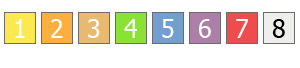
\includegraphics[width=.75\textwidth]{./imagenes/Casillas.jpg}
\caption{Casillas}
\end{center}
Algunas casillas tienen un número y color especifico, este número indica las minas que suman todas las casillas circundantes.Así, si una casilla tiene el número 3, significa que de las ocho casillas que hay alrededor (si no es en una esquina o borde) hay 3 con minas y 5 sin minas. Si se descubre una casilla sin número indica que ninguna de las casillas vecinas tiene mina y estas se descubren automáticamente.
\end{figure}
 
\ \\ 
\begin{figure}[htbp]
\begin{center}
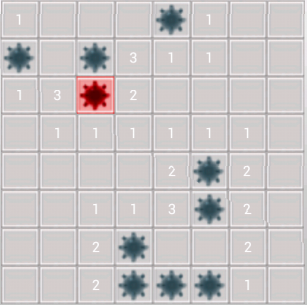
\includegraphics[width=.45\textwidth]{./imagenes/minas.png}
\caption{Perdio juego}
\end{center}
Si se descubre una casilla con una mina se pierde la partida
\end{figure}
\ \\ 
\begin{figure}[htbp]
\begin{center}

\includegraphics[width=.35\textwidth]{./imagenes/casilla_bandera.png}
\caption{Perdio juego}
\end{center}
Se puede poner una marca en las casillas que el jugador piensa que hay minas para ayudar a descubrir la que están cerca.
\end{figure}
\ \\ 
\begin{figure}[htbp]
\begin{center}
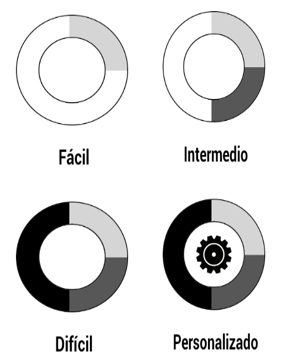
\includegraphics[width=.50\textwidth]{./imagenes/Niveles.png}
\caption{Perdio juego}
\end{center}
El juego también posee un sistema de récords para cada uno de Los 4 niveles en el que se indica el menor tiempo en terminar el juego.Los niveles son:
\\Nivel Facil: 8 x 8 casillas y 10 minas.
\\Nivel Intermedio: 10 x 10 casillas y 15 minas.
\\Nivel Dificil: 12 x 12 casillas y 20 minas.
\\Nivel Personalizado: en este caso el usuario personaliza su juego eligiendo el número de minas y el tamaño de la cuadricula.
\end{figure}
